\documentclass{beamer}
\usetheme{Madrid}
\usepackage{array}
\setbeamertemplate{caption}[numbered]
\title[CST 309 M1]{MANAGEMENT OF SOFTWARE SYSTEMS}
\subtitle{Module 1}
\author{Rijin IK}
\institute[VJEC]{Assistant Professor\\Department of Computer Science and Engineering\\Vimal Jyothi Engineering College\\Chemperi}
\begin{document}
	\begin{frame}
		\titlepage
	\end{frame}
   \begin{frame}{Outline}
   \tableofcontents
   \end{frame}
\section{Introduction to Software Engineering}
\begin{frame}{Introduction to Software Engineering}
\begin{block}{Software Engineering}
	\begin{itemize}
		\item Software engineering is the branch of computer science that deals with the design, development, testing, and maintenance of software applications.
		\item Software engineers apply engineering principles and knowledge of programming languages to build software solutions for end users.
	\end{itemize}
\end{block}
\end{frame}
\begin{frame}{Frequently 
		asked questions about 
		software engineering}
\textbf{What is Software?}
\begin{itemize}
	\item Computer programs and associated 
	documentation.
	\item Software products may be 
	developed for a particular customer or 
	may be developed for a general market.
\end{itemize}
\textbf{What are the Attributes of good software?}
\begin{itemize}
	\item Good software should deliver the required 
	functionality and performance to the user 
	\item And should be maintainable, dependable 
	and usable
\end{itemize}
\textbf{What is Software engineering?}
\begin{itemize}
	\item Software engineering is an engineering 
	discipline that is concerned with all 
	aspects of software production.
	\item  from initial conception to 
	operation and maintenance.
\end{itemize}
\end{frame}
\begin{frame}{Frequently 
		asked questions about 
		software engineering}
\textbf{What are the Fundamental software 
	engineering activities?}
\begin{itemize}
	\item Software specification
	\item Software development 
	\item Software validation 
	\item software evolution.
\end{itemize}
\textbf{What is the Difference between software 
	engineering and computer science}
\begin{itemize}
	\item Computer science focuses on theory and 
	fundamentals; 
	\item software engineering is 
	concerned with the practicalities of 
	developing and delivering useful 
	software.
\end{itemize}
\end{frame}
\begin{frame}{Frequently 
		asked questions about 
		software engineering}
\textbf{Difference between software 
	engineering and system engineering}
\begin{itemize}
	\item System engineering is concerned with all 
	aspects of computer-based systems 
	development including hardware, 
	software and process engineering. 
	Software engineering is part of this more 
	general process.
	
\end{itemize}
\textbf{What are the Key challenges facing 
	software engineering}
\begin{itemize}
	\item Coping with increasing diversity
	\item Demands for reduced delivery times 
	\item Developing trustworthy software
\end{itemize}
\textbf{What are the Costs of software 
	engineering}
\begin{itemize}
	\item Roughly 60\%\  of software costs are 
	development costs, 40\%\  are testing costs. 
	\item For custom software, evolution costs 
	often exceed development costs.
\end{itemize}
\end{frame}
\begin{frame}{Frequently 
		asked questions about 
		software engineering}
	\textbf{What are the Best software engineering 
		techniques and methods}
	\begin{itemize}
		\item While all software projects have to be 
		professionally managed and developed, 
		different techniques are appropriate for 
		different types of system. For example, 
		games should always be developed using 
		a series of prototypes whereas safety 
		critical control systems require a complete 
		and analyzable specification to be 
		developed. 
		\item You can’t, therefore, say that 
		one method is better than another.
	\end{itemize}

\textbf{What differences has the Internet 
	made to software engineering?}
\begin{itemize}
	\item Not only has the Internet led to the development of massive, highly 
	distributed, service-based systems, it has also supported the 
	creation of an “app” industry for mobile devices which has 
	changed the economics of software.
\end{itemize}
\end{frame}

\begin{frame}{Professional software development}
\textbf{Professional software development}
\begin{itemize}
	\item Software development is a professional activity in which software is developed 
	\begin{itemize}
		\item for business purposes.
		\item for inclusion in other devices.
		\item as software products.
	\end{itemize}
\item Professional software is intended for use by someone apart from its developer.
\item It is maintained and changed throughout its life.
\item It includes techniques that support program \textbf{specification, design, and evolution},    none of which are normally relevant for personal software development.
\end{itemize}
\end{frame}
\section{Professional software development}
\begin{frame}{Professional software development}
	\begin{itemize}
		\item Software is not just the programs themselves but also all associated 
		\begin{itemize}
			\item documentation, 
			\item libraries, 
			\item support websites,
			\item configuration data that are needed to make these programs useful.
		\end{itemize}
	\item A system may consist of several separate programs and configuration files that are    used to set up these programs. It may include 
	\begin{itemize}
		\item System documentation, which describes the structure of the system. 
		\item User documentation, which explains how to use the system.
		\item Websites for users to download recent product information.
	
	\end{itemize}
	\item Software engineers are concerned with developing software products, that is, software      that can be sold to a customer. 
	\end{itemize}
\end{frame}
\begin{frame}{Professional software development}
	\textbf{Essential attributes of good software}
	\begin{itemize}
		\item Maintainability
		\begin{itemize}
			\item Software should be written in such a way so that it can evolve to meet the changing needs of customers.
			This is a critical attribute because software change is an inevitable requirement of a changing business environment.		
		\end{itemize}
		\item Dependability and security
		\begin{itemize}
			\item Software dependability includes a range of characteristics including reliability, security and safety.
			Dependable software should not cause physical or economic damage in the event of system failure. Malicious users should not be  able to access or damage the system.
		\end{itemize}
		\item Efficiency
		\begin{itemize}
			\item Software should not make wasteful use of system resources such as memory and processor cycles. 
			Efficiency therefore includes responsiveness, processing time, memory utilisation, etc.
		\end{itemize}
		\item Acceptability
		\begin{itemize}
			\item Software must be acceptable to the type of users for which it is designed. 
			This means that it must be understandable, usable and compatible with other systems that they use.
		\end{itemize}
	\end{itemize}
\end{frame}
\begin{frame}{Professional software development}
	\textbf{Software products:-}There are two kinds of software product
	\begin{enumerate}
		\item Generic products.
		\begin{itemize}
			\item These are stand-alone systems that are produced by a development organization and sold on the open market to any customer who is able to buy them.
			\item mobile apps 
		\end{itemize}
	\item Customized software.
	\begin{itemize}
		\item These are systems that are commissioned by and developed for a particular      customer.
		\item A software contractor designs and implements the software especially for that  customer.
		
	\end{itemize}
	\end{enumerate}
\end{frame}
\begin{frame}{Professional software development}
	\textbf{Software engineering}
	\begin{itemize}
		\item Software engineering is an engineering discipline that is concerned with all aspects of    software production from the early stages of system specification through to maintaining the system after it has gone into use.
		\item Two key phrases: 
		\begin{enumerate}
			\item \textbf{Engineering discipline.}
			\begin{itemize}
				\item Using appropriate theories and methods to solve problems within the 
				organizational and financial constraints.
			\end{itemize}
		\item \textbf{All aspects of software production} 
	
		\begin{itemize}
				\item Software engineering is not just concerned with the technical processes of software development. 
			\item It also includes activities such as software project management and the           development of tools, methods, and theories to support software development.
		\end{itemize}
		\end{enumerate}
	\end{itemize}
\end{frame}
\begin{frame}{Professional software development}
	\textbf{Why software engineering is important? }\\
\ \ 	Software engineering is important for two reasons:
\begin{enumerate}
	\item More and more, individuals and society rely on advanced software systems.
	\begin{itemize}
		\item We need to be able to produce reliable and trustworthy systems economically and quickly.
	\end{itemize} 
	\item It is usually cheaper, in the long run, to use software engineering methods and 
	techniques for professional software systems rather than just write programs as a       
	personal programming project. 
	
\end{enumerate}
Failure to use software engineering method leads to higher costs for testing, quality assurance, and long-term maintenance.	
\end{frame}
\begin{frame}{Professional software development}
\begin{block}{SOFTWARE PROCESS}
The systematic approach that is used in software engineering is sometimes called 
a software process. A software process is a sequence of activities that leads to the 
production of a software product.
\end{block}
Four fundamental activities are common to all software processes.
\begin{enumerate}
	\item \textbf{Software specification}, where customers and engineers define the software that
	is to be produced and the constraints on its operation.
	\item \textbf{Software development}, where the software is designed and programmed.
	\item \textbf{Software validation}, where the software is checked to ensure that it is what the customer requires.
	\item \textbf{Software evolution}, where the software is modified to reflect changing customer and market requirements.
\end{enumerate}
\end{frame}
\begin{frame}{Professional software development}
\textbf{General issues that affect most Software}
\begin{enumerate}
	\item Heterogeneity:
	\begin{itemize}
		\item Operating in a distributed systems across networks that include different types of     computer and mobile devices, it is often have to integrate new software with older   systems written in different programming languages.
	\end{itemize}
	\item Business and social change:
	\begin{itemize}
		\item Many traditional software engineering techniques are time consuming, and delivery of new systems often takes longer than planned. But it is needed to change their       existing software and to rapidly develop new software.
	\end{itemize}
	\item Security and trust:
	\begin{itemize}
		\item We have to make sure that malicious users cannot successfully attack our software  and that information security is maintained.
	\end{itemize}
	\item Scale:
	\begin{itemize}
		\item Software has to be developed across a very wide range of scales, from very small    embedded systems in portable or wearable devices through to Internet-scale, cloud-based systems that serve a global community.
	\end{itemize}
\end{enumerate}
\end{frame}

\begin{frame}{{Professional software development}}
\textbf{Software Engineering Diversity}
\begin{itemize}
	\item There are many different types of software system and there is no universal set of software techniques that is applicable to all of these.

	\item The software engineering methods and tools used depend on the type of application 
	being developed, the requirements of the customer and the background of the 
	development team.
\end{itemize}
\end{frame}
\begin{frame}{{Professional software development}}
	\textbf{Application types}
	\begin{itemize}
		\item Stand-alone applications 
		\begin{itemize}
			\item These are application systems that run on a local computer, such as a PC. They include all necessary functionality and do not need to be connected to a 
			network.
		\end{itemize}
	\item Interactive transaction-based applications
	\begin{itemize}
		\item Applications that execute on a remote computer and are accessed by users from 
		their own PCs or terminals. These include web applications such as e-commerce 
		applications. 
	\end{itemize}
\item Embedded control systems
\begin{itemize}
	\item These are software control systems that control and manage hardware devices. 
	Numerically, there are probably more embedded systems than any other type of 
	system.

\end{itemize}
	\end{itemize}
\end{frame}
\begin{frame}{{Professional software development}}
	\textbf{Application types cont..}
	\begin{itemize}
		\item Batch processing systems
		\begin{itemize}
			\item These are business systems that are designed to process data in large batches. 
			They process large numbers of individual inputs to create corresponding 
			outputs. 
		\end{itemize}
		\item Entertainment systems 
		\begin{itemize}
			\item These are systems that are primarily for personal use and which are intended to entertain the user. 
		\end{itemize}
		\item Systems for modeling and simulation
		\begin{itemize}
			\item These are systems that are developed by scientists and engineers to model 
			physical processes or situations, which include many, separate, interacting 
			objects.
		\end{itemize}
	\end{itemize}
\end{frame}

\begin{frame}{{Professional software development}}
	\textbf{Application types cont..}
	\begin{itemize}
		\item Data collection systems
		\begin{itemize}
			\item These are systems that collect data from their environment using a set of sensors and send that data to other systems for processing.
		\end{itemize}
		\item Systems of systems 
		\begin{itemize}
			\item  These are systems that are composed of a number of other software systems.
			\item Software that has already been developed rather than write new software.

		\end{itemize}
	\end{itemize}
\end{frame}

\begin{frame}{{Professional software development}}
	\textbf{Software Engineering and the Web}
	\begin{itemize}
		\item The Web is now a platform for running application and organizations are increasingly developing web-based systems rather than local systems.
		\item Web services allow application functionality to be accessed over the web.
		\item Cloud computing is an approach to the provision of computer services where applications run remotely on the ‘cloud’. 
		
		\begin{itemize}
			\item Users do not buy software buy pay according to use
			
	
		\end{itemize}

	\end{itemize}
\end{frame}
\begin{frame}{{Professional software development}}
	\textbf{Web software Engineering}
	\begin{itemize}
			\item Software reuse is the dominant approach for constructing web-based systems. 	
		\begin{itemize}
			\item When building these systems, you think about how you can assemble them from pre-existing software components and systems.
		\end{itemize}
		\item Web-based systems should be developed and delivered incrementally.
		\begin{itemize}
			\item It is now generally recognized that it is impractical to specify all the requirements for such systems in advance. 
		\end{itemize}
		\item User interfaces are constrained by the capabilities of web browsers. 
		\begin{itemize}
			\item Technologies such as AJAX allow rich interfaces to be created within a web browser but are still difficult to use. Web forms with local scripting are more commonly used. 
		\end{itemize}
	\end{itemize}
\end{frame}
\begin{frame}{{Professional software development}}
	\textbf{Web based Software Engineering}
	\begin{itemize}
		\item Web-based systems are complex distributed systems but the fundamental principles of 
		software engineering discussed previously are as applicable to them as they are to any other types of system
		\item The fundamental ideas of software engineering, discussed in the previous section, 
		apply to web-based software in the same way that they apply to other types of software system.
	\end{itemize}
\end{frame}
\section{Software engineering ethics}
\begin{frame}{Software engineering ethics}
	\textbf{Software engineering ethics}
\begin{itemize}
	\item Software engineering involves wider responsibilities than simply the application of technical skills.
	\item Software engineers must behave in an honest and ethically responsible way if they are to be respected as professionals.
	\item Ethical behaviour is more than simply upholding the law but involves following a set of principles that are morally correct.
\end{itemize}
\end{frame}
\begin{frame}{Software engineering ethics}
	\textbf{Issues of Professional Responsibility}
	\begin{itemize}
		\item Confidentiality 
		\begin{itemize}
			\item Engineers should normally respect the confidentiality of their employers or clients irrespective of whether or not a formal confidentiality agreement has been signed.

		\end{itemize}
	  \item Competence 
	  \begin{itemize}
	  	\item Engineers should not misrepresent their level of competence. They should not 
	  	knowingly accept work which is outwith their competence.

	  \end{itemize}
  \item Intellectual property rights
  \begin{itemize}
  	\item Engineers should be aware of local laws governing the use of intellectual 
  	property such as patents, copyright, etc. They should be careful to ensure that 
  	the intellectual property of employers and clients is protected.

  \end{itemize}
\item Computer misuse
\begin{itemize}
	\item Software engineers should not use their technical skills to misuse other people’s 
	computers. Computer misuse ranges from relatively trivial (game playing on an 
	employer’s machine, say) to extremely serious (dissemination of viruses).
\end{itemize}
	\end{itemize}
\end{frame}
\begin{frame}{Software engineering ethics}
\textbf{ACM/IEEE Code of Ethics}
\begin{itemize}
	\item The professional societies in the US have cooperated to produce a code of ethical 
	practice.
	\item Members of these organisations sign up to the code of practice when they join
	\item The Code contains eight Principles related to the behaviour of and decisions made by professional software engineers, including practitioners, educators, managers, 
	supervisors and policy makers, as well as trainees and students of the profession. 
\end{itemize}
\end{frame}
\begin{frame}{ACM/IEEE Code of Ethics}
\textbf{Software Engineering Code of Ethics and Professional Practice}
\begin{itemize}
	\item ACM/IEEE-CS Joint Task Force on Software Engineering Ethics and Professional Practices
\end{itemize}
\textbf{PREAMBLE}
\begin{itemize}
	\item The short version of the code summarizes aspirations at a high level of the abstraction; the clauses that are included in the full version give examples and details of how these aspirations change the way we act as software engineering professionals. Without the aspirations, the details can become legalistic and tedious; without the details, the aspirations can become high sounding but empty; together, the aspirations and the details form a cohesive code.
	\item Software engineers shall commit themselves to making the analysis, specification, design, development, testing and maintenance of software a beneficial and respected profession. In accordance with their commitment to the health, safety and welfare of the public, software engineers shall adhere to the following Eight Principles:
	
\end{itemize}
\end{frame}
\begin{frame}{ACM/IEEE Code of Ethics}
	\textbf{Ethical principles}
	\begin{itemize}
		\item[1] \textbf{PUBLIC} — Software engineers shall act consistently with the public interest.
		\item[2] \textbf{ CLIENT AND EMPLOYER} — Software engineers shall act in a manner that is in the 
		best interests of their client and employer consistent with the public interest.
		\item[3] \textbf{ PRODUCT} — Software engineers shall ensure that their products and related 
		modifications meet the highest professional standards possible.
		\item[4] \textbf{ JUDGMENT} — Software engineers shall maintain integrity and independence in their 
		professional judgment.
			\item[5] \textbf{ MANAGEMENT} — Software engineering managers and leaders shall subscribe to and 
		promote an ethical approach to the management of software development and 
		maintenance.
		
	\end{itemize}
\end{frame}
\begin{frame}{ACM/IEEE Code of Ethics}
	\textbf{Ethical principles cont...}
	\begin{itemize}
		\item[6] \textbf{PROFESSION} — Software engineers shall advance the integrity and reputation of 
	the profession consistent with the public interest.
	\item[7] \textbf{COLLEAGUES} — Software engineers shall be fair to and supportive of their 
	colleagues.
	\item[8] \textbf{SELF} — Software engineers shall participate in lifelong learning regarding 
	the practice of their profession and shall promote an ethical approach to the 
	practice of the profession
	\end{itemize}
\end{frame}
\begin{frame}{ACM/IEEE Code of Ethics}
	\textbf{Rationale for the code of ethics}
	\begin{itemize}
		\item Computers have a central and growing role in commerce, industry, government, medicine, education, entertainment and society at large. Software engineers are those who contribute by direct participation or by teaching, to the analysis, specification, design, development, certification, maintenance and testing of software systems. 
		\item Because of their roles in developing software systems, software engineers have significant opportunities to do good or cause harm, to enable others to do good or cause harm, or to influence others to do good or cause harm. To ensure, as much as possible, that their efforts will be used for good, software engineers must commit themselves to making software engineering a beneficial and respected profession. 
		
	\end{itemize}
\end{frame}
\section{Case Studies}
\begin{frame}{Case Studies}
	\begin{itemize}
		\item A personal insulin pump
		\begin{itemize}
			\item An embedded system in an insulin pump used by diabetics to maintain blood glucose control.
		\end{itemize}
		\item A mental health case patient management system
		\begin{itemize}
			\item A system used to maintain records of people receiving care for mental health problems.
		\end{itemize}
		\item A wilderness weather station
	   \begin{itemize}
	   	\item 	A data collection system that collects data about weather conditions in remote areas
	   \end{itemize}
	\end{itemize}
\end{frame}
\begin{frame}{Insulin pump control system}
	An insulin pump is a medical system that simulates the operation of the pancreas (an 
	internal organ). The software controlling this system is an embedded system that 
	collects information from a sensor and controls a pump that delivers a controlled 
	dose of insulin to a user.
\begin{itemize}
	\item Collects data from a blood sugar sensor and calculates the amount of insulin required to be injected.
	\item Calculation based on the rate of change of blood sugar levels.
	\item Sends signals to a micro-pump to deliver the correct dose of insulin.
	\item Safety-critical system as low blood sugars can lead to brain malfunctioning, coma and death; high-blood sugar levels have long-term consequences such as eye and kidney damage.
	
\end{itemize}
\end{frame}
\begin{frame}{Insulin pump control system}
\begin{figure}
	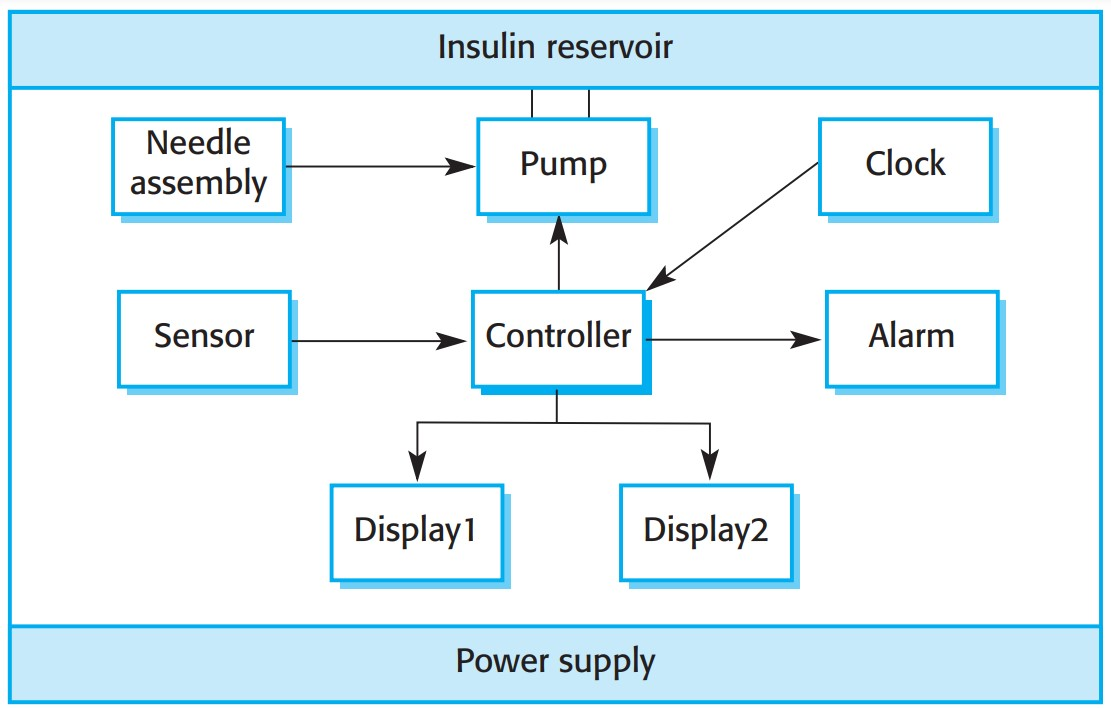
\includegraphics[scale=.4]{img/m1_1.jpg}
	\caption{Insulin pump 
		hardware architecture}
\end{figure}
\end{frame}
\begin{frame}{Insulin pump control system}
	\begin{figure}
		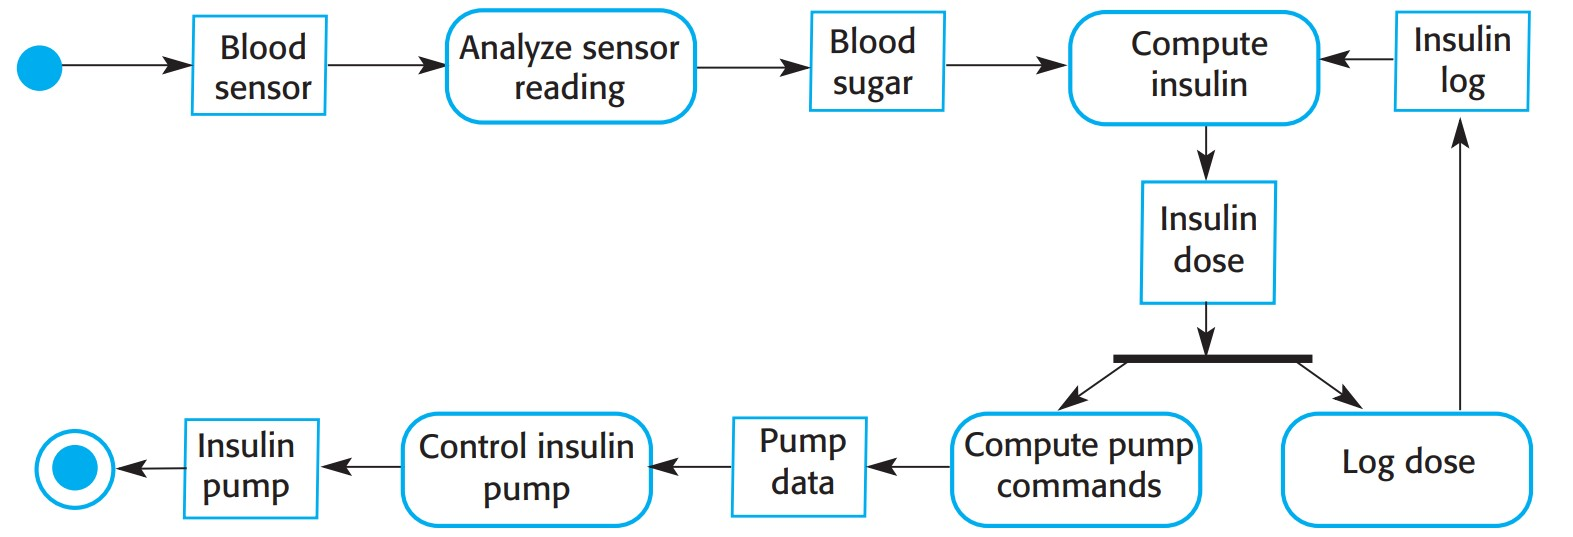
\includegraphics[scale=.35]{img/m1_2.jpg}
		\caption{Activity 
			model of the 
			insulin pump}
	\end{figure}
\end{frame}
\begin{frame}{Insulin pump control system}
	\textbf{Essential high-level requirements}
	\begin{itemize}
		\item The system shall be available to deliver insulin when required. 
		\item The system shall perform reliably and deliver the correct amount of insulin to counteract the current level of blood sugar.
		\item The system must therefore be designed and implemented to ensure that the system always meets these requirements. 
	\end{itemize}
\end{frame}
\begin{frame}{A Patient Information System for Mental Health Care}
\begin{itemize}
	\item A patient information system to support mental health care is a medical information system that maintains information about patients suffering from mental health problems and the treatments that they have received.
	\item Most mental health patients do not require dedicated hospital treatment but need to attend specialist clinics regularly where they can meet a doctor who has detailed knowledge of their problems. 
	\item To make it easier for patients to attend, these clinics are not just run in hospitals. They may also be held in local medical practices or community centres. 
	
\end{itemize}
\end{frame}
\begin{frame}{A Patient Information System for Mental Health Care}
	\begin{itemize}
		\item The \textbf{MHC-PMS (Mental Health Care-Patient Management System)} is an information 
		system that is intended for use in clinics.
		\item It makes use of a centralized database of patient information but has also been designed 
		to run on a PC, so that it may be accessed and used from sites that do not have secure 
		network connectivity. 
		\item When the local systems have secure network access, they use patient information in the 
		database but they can download and use local copies of patient records when they are 
		disconnected.
	\end{itemize}
\end{frame}
\begin{frame}{A Patient Information System for Mental Health Care}
	\textbf{MHC-PMS goals}
	\begin{itemize}
		\item To generate management information that allows health service managers to assess 
		performance against local and government targets.
		\item To provide medical staff with timely information to support the treatment of patients.
		The organization of the MHC-PMS
	\end{itemize}
\end{frame}
\begin{frame}{A Patient Information System for Mental Health Care}
	\begin{figure}
		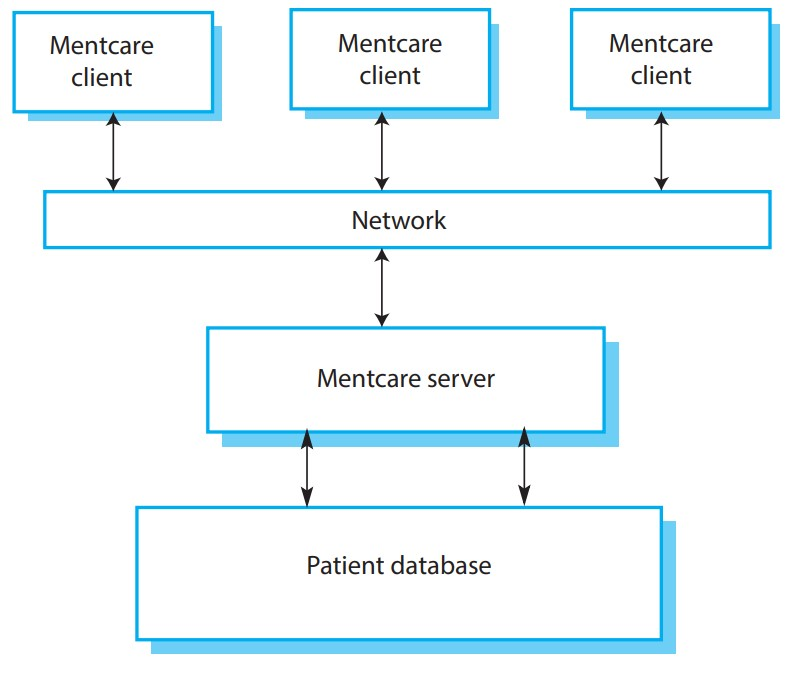
\includegraphics[scale=.45]{img/m1_3.jpg}
		\caption{The 
			organization of the 
			Mentcare system}
	\end{figure}
\end{frame}
\begin{frame}{A Patient Information System for Mental Health Care}
\textbf{MHC-PMS key features}
\begin{itemize}
	\item \textbf{Individual care management} 
	\begin{itemize}
		\item Clinicians can create records for patients, edit the information in the system, view patient history, etc. The system supports data summaries so that doctors can quickly learn about the key problems and treatments that have been prescribed.
	\end{itemize}
	
	\item \textbf{Patient monitoring}
	\begin{itemize}
		\item The system monitors the records of patients that are involved in treatment and issues warnings if possible problems are detected. 
	\end{itemize} 

\item	\textbf{Administrative reporting}
	\begin{itemize}
		\item The system generates monthly management reports showing the number of patients treated at each clinic, the number of patients who have entered and left the care system, number of patients sectioned, the drugs prescribed and their costs, etc. 
	\end{itemize} 
\end{itemize}
\end{frame}
\begin{frame}{A Patient Information System for Mental Health Care}
	\textbf{MHC-PMS concerns}
	\begin{itemize}
		\item Privacy
	\begin{itemize}
		\item It is essential that patient information is confidential and is never disclosed to anyone apart from authorised medical staff and the patient themselves. 
	\end{itemize}
		\item Safety
		\begin{itemize}
			\item Some mental illnesses cause patients to become suicidal or a danger to other people. Wherever possible, the system should warn medical staff about potentially suicidal or dangerous patients. 
			\item The system must be available when needed otherwise safety may be compromised and it may be impossible to prescribe the correct medication to patients. 
		\end{itemize}
	\end{itemize}
\end{frame}
\begin{frame}{Wilderness weather station}
	\textbf{Wilderness weather station}
\begin{itemize}
	\item The government of a country with large areas of wilderness decides to deploy several hundred weather stations in remote areas. 
	\item Weather stations collect data from a set of instruments that measure temperature and pressure, sunshine, rainfall, wind speed and wind direction.

	\begin{itemize}
		\item The weather station includes a number of instruments that measure weather parameters such as the wind speed and direction, the ground and air temperatures, the barometric pressure and the rainfall over a 24-hour period. 
		\item Each of these instruments is controlled by a software system that takes parameter readings periodically and manages the data collected from the instruments.  
	\end{itemize}
\end{itemize}
\end{frame}
\begin{frame}{Wilderness weather station}
	\begin{figure}
		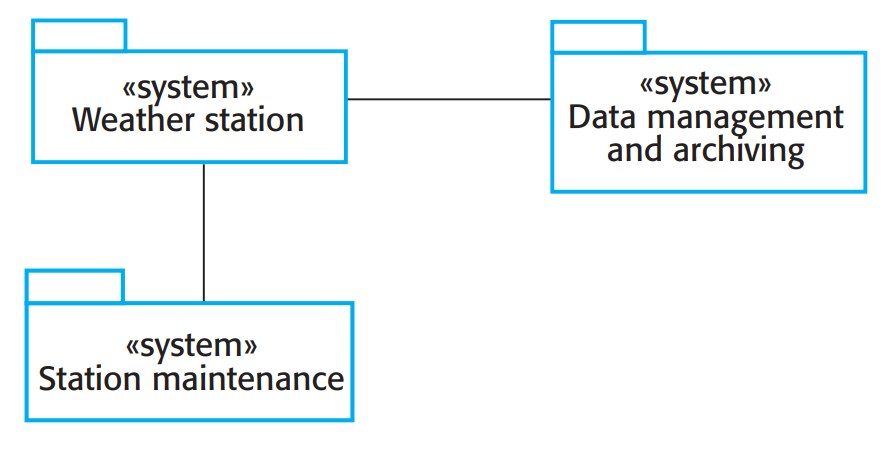
\includegraphics[scale=.45]{img/m1_4.jpg}
		\caption{The weather 
			station’s environment}
	\end{figure}
\end{frame}
\begin{frame}{Wilderness weather station}
	
\textbf{The weather station system }
\begin{itemize}
	\item This is responsible for collecting weather data, carrying out some initial data 
	processing and transmitting it to the data management system.
\end{itemize}
\textbf{The data management and archiving system }
\begin{itemize}
	\item This system collects the data from all of the wilderness weather stations, carries out 
	data processing and analysis and archives the data.
\end{itemize}
\textbf{The station maintenance system }
\begin{itemize}
	\item This system can communicate by satellite with all wilderness weather stations to 
	monitor the health of these systems and provide reports of problems.
\end{itemize}
\end{frame}
\begin{frame}{Wilderness weather station}
	
	\textbf{Additional software functionality}
	\begin{itemize}
		\item Monitor the instruments, power and communication hardware and report faults to the management system.
		\item Manage the system power, ensuring that batteries are charged whenever the environmental conditions permit but also that generators are shut down in potentially damaging weather conditions, such as high wind.
		\item Support dynamic reconfiguration where parts of the software are replaced with new versions and where backup instruments are switched into the system in the event of system failure.
	\end{itemize}
\end{frame}
\section{Software process models}
\begin{frame}{The software process}
	\textbf{The software process}
	\begin{itemize}
		\item A structured set of activities required to develop a software system. 
		\item Many different software processes but all involve:
		\begin{itemize}
			\item \textbf{Specification} – defining what the system should do;
			\item \textbf{Design and implementation} – defining the organization of the system and implementing the system;
			\item \textbf{Validation} – checking that it does what the customer wants;
			\item \textbf{Evolution} – changing the system in response to changing customer needs.
		\end{itemize}
	\item A software process model is an abstract representation of a process. It presents a description of a process from some particular perspective
	\end{itemize}
\end{frame}
\begin{frame}{The software process}
	\textbf{Software process descriptions:}
		When we describe and discuss processes, we usually 
	talk about the activities in these processes such as 
	specifying a data model, designing a user interface, etc. 
	and the ordering of these activities.
	\begin{itemize}

	\item Process descriptions may also include
		\begin{itemize}
			\item \textbf{Products}, which are the outcomes of a process activity; 
			\item \textbf{Roles}, which reflect the responsibilities of the people involved in the process;
			\item \textbf{Pre- and post-conditions}, which are statements that are true before and after a process activity has been enacted or a product produced.   
			
		\end{itemize}
	\end{itemize}
\end{frame}
\begin{frame}{The software process}
	\textbf{Plan-driven and agile processes}
\begin{itemize}
	\item Plan-driven processes are processes where all of the 
	process activities are planned in advance and progress 
	is measured against this plan. 
	\item In agile processes, planning is incremental and it is 
	easier to change the process to reflect changing 
	customer requirements. 
	\item In practice, most practical processes include elements of 
	both plan-driven and agile approaches. 
	\item There are no right or wrong software processes.
\end{itemize}
\end{frame}
\begin{frame}{Software process models}
	\textbf{Software process models}
	\begin{itemize}
		\item Sometimes called a Software Development Life Cycle (SDLC model)
		\item a simplified representation of a software process. 
		\item Each process model represents a process from a particular perspective and thus only provides partial information about that process. 
		\item For example, a process activity model shows the activities and their sequence but may not show the roles of the people involved in these activities.
		\item The general process models (sometimes called process paradigms)
			\begin{enumerate}
			\item The waterfall model
			\item Incremental development	
			\item Integration and configuration
		\end{enumerate}
	\end{itemize}
\end{frame}
\begin{frame}{THE WATERFALL MODEL}
	\begin{block}{The Waterfall model }
	This takes the fundamental process activities of specification, development, validation, and evolution and represents them as separate process phases such as 
	\begin{itemize}
		\item Requirements specification
		\item software design
		\item Implementation
		\item testing.
	\end{itemize}
	\end{block}
\begin{itemize}
	\item The first published model of the software development process
	\item The waterfall model is an example of a plan-driven process
	\item Plan and schedule all of the process activities before starting software development.
\end{itemize}
\end{frame}
\begin{frame}{THE WATERFALL MODEL}
\begin{figure}
	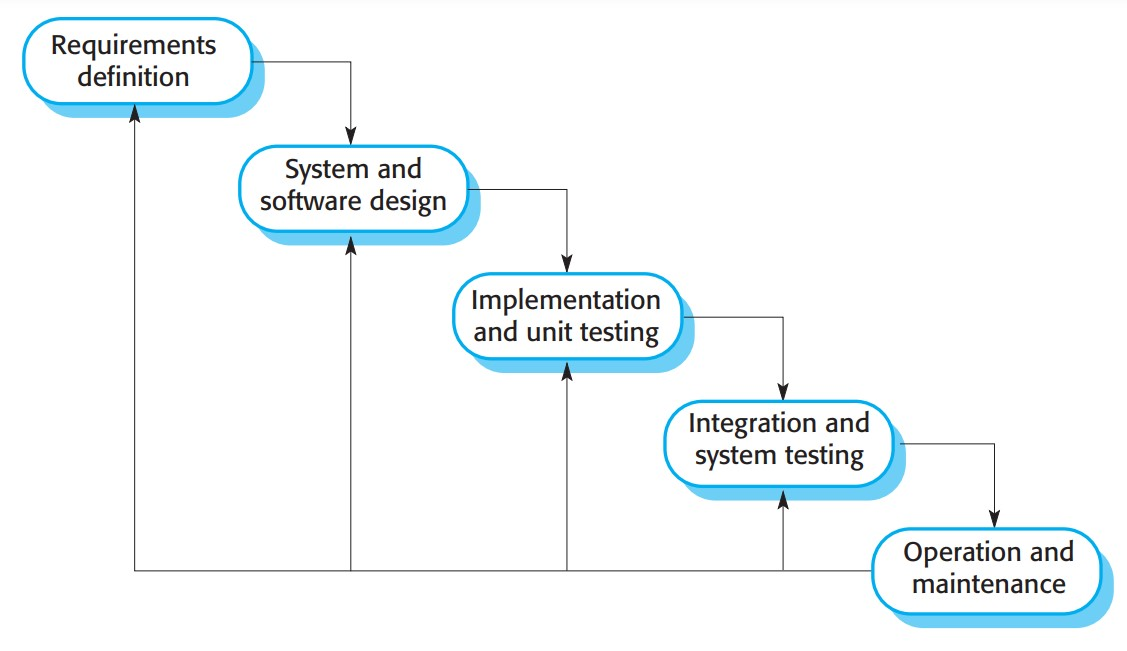
\includegraphics[scale=.45]{img/m1_5.jpg}
	\caption{The Waterfall model}
\end{figure}
\end{frame}
\begin{frame}{THE WATERFALL MODEL}
Activities are,
\begin{itemize}
	\item[1] \textbf{Requirements analysis and definition} The system’s services, constraints, and goals are established   by consultation with system users. They are then defined in detail and serve as a system specification.
	\item[2] \textbf{ System and software design} The systems design process allocates the requirements to either hardware or software systems. It establishes an overall system architecture. Software design involves identifying and describing the fundamental software system abstractions and their relationships.
	\item[3] \textbf{Implementation and unit testing} During this stage, the software design is realized as a set of programs or program units. Unit testing involves verifying that each unit meets its specification.
	
\end{itemize}
\end{frame}
\begin{frame}{THE WATERFALL MODEL}
	\begin{itemize}
		\item[4] \textbf{Integration and system testing} The individual program units or programs are integrated and tested as a complete system to ensure that the software requirements have been met. After testing, the software system is delivered to the customer.
		\item[5] \textbf{Operation and maintenance} Normally, this is the longest life-cycle phase. The system is installed and put into practical use. Maintenance involves correcting errors that were not discovered in earlier stages of the life cycle, improving the implementation of system units, and enhancing the system’s services as new requirements are discovered.
	\end{itemize}
\end{frame}
\begin{frame}{THE WATERFALL MODEL}
\textbf{Waterfall Model Problems:}
\begin{itemize}
	\item The main drawback of the waterfall model is the difficulty of accommodating change after 
	the process is underway. In principle, a phase has to be complete before moving onto the 
	next phase.
	\item Inflexible partitioning of the project into distinct stages makes it difficult to respond to changing customer requirements.
	\begin{itemize}
		\item Therefore, this model is only appropriate when the requirements are well-understood and changes will be fairly limited during the design process. 
		\item Few business systems have stable requirements.
	\end{itemize}
\item The waterfall model is mostly used for large systems engineering projects where a 
system is developed at several sites.
\begin{itemize}
	\item In those circumstances, the plan-driven nature of the waterfall model helps 
	coordinate the work. 
	
\end{itemize}
\end{itemize}
\end{frame}
\begin{frame}{INCREMENTAL DEVELOPMENT}
\textbf{Incremental Development}
\begin{itemize}
	\item This approach interleaves the activities of specification, development, and validation. 
	\item The system is developed as a series of versions (increments), with each version adding functionality to the previous version.
\end{itemize}
	\begin{figure}
	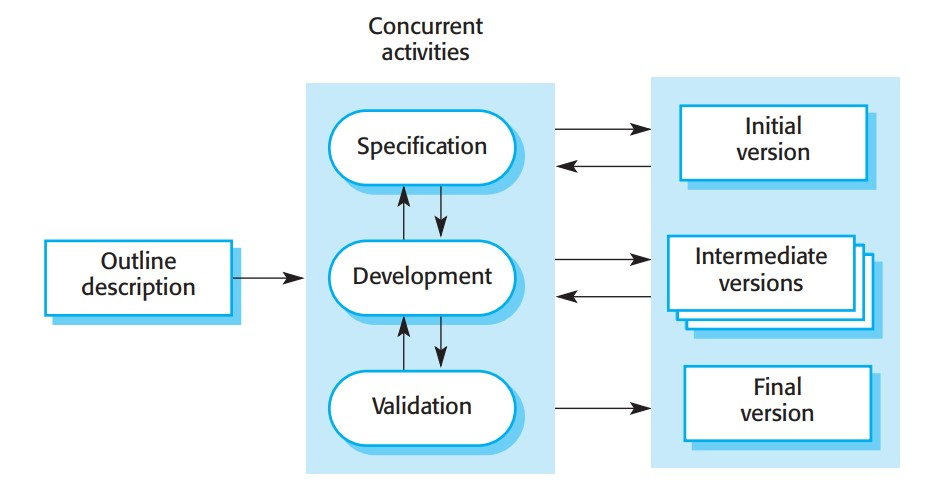
\includegraphics[scale=.45]{img/m1_6.jpg}
	\caption{Incremental 
		development}
\end{figure}
\end{frame}
\begin{frame}{INCREMENTAL DEVELOPMENT}
	\textbf{Incremental development has three major advantages over the waterfall model:}
	\begin{enumerate}
		\item The cost of accommodating changing customer requirements is reduced. 
		\begin{itemize}
			\item The amount of analysis and documentation that has to be redone is much less than is required with the waterfall model.
		\end{itemize}
	\item It is easier to get customer feedback on the development work that has been done.
	\begin{itemize}
		\item Customers can comment on demonstrations of the software and see how much 
		has been implemented.
	\end{itemize}
\item Early delivery and deployment of useful software to the customer is possible, 
even if all of the functionality has not been included.
\begin{itemize}
	\item Customers are able to use 
	and gain value from the software earlier than is possible with a waterfall process.
\end{itemize} 
	\end{enumerate}
\end{frame}
\begin{frame}{INCREMENTAL DEVELOPMENT}
	\textbf{From a management perspective, the incremental approach has two problems:}
	\begin{enumerate}
		\item The process is not visible. 
		\begin{itemize}
			\item Managers need regular deliverables to measure progress.       If systems are developed quickly, it is not cost effective to produce documents that reflect every version of the system.
		\end{itemize}
	\item System structure tends to degrade as new increments are added.
	\begin{itemize}
		\item Regular change leads  to messy code as new functionality is added in whatever way is possible. It becomes increasingly difficult and costly to add new features to a system. 
	\end{itemize}
	\end{enumerate}
\end{frame}
\begin{frame}{INTEGRATION AND CONFIGURATION}
\textbf{INTEGRATION AND CONFIGURATION(Reuse-oriented software engineering)}
\begin{itemize}
	\item This approach relies on the availability of reusable components or systems. 
	\item The system development process focuses on configuring these components for use in a new setting and integrating them into a system.
\end{itemize}
\begin{figure}
		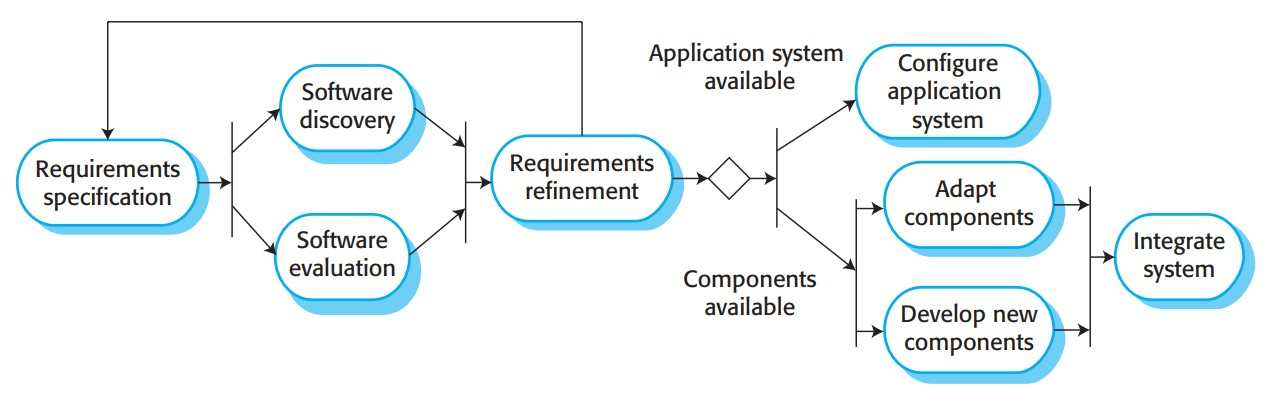
\includegraphics[scale=.4]{img/m1_7.jpg}
	\caption{Reuse oriented software 
		engineering}
\end{figure}
\end{frame}
\begin{frame}{INTEGRATION AND CONFIGURATION}
\begin{itemize}
	\item This often happens informally when people working on the project know of or search for code that is similar to what is required. 
	\item They look for these, modify them as needed, and integrate them with the new code that they have developed.
	\item Three types of software components are frequently reused:
	\begin{enumerate}
		\item Stand-alone application systems that are configured for use in a particular environment. These systems are general-purpose systems that have many features, but they have to be adapted for use in a specific application.
		
		\item Collections of objects that are developed as a component or as a package to be integrated with a component framework.
		
		\item Web services that are developed according to service standards and that are available for remote invocation over the Internet.
	\end{enumerate}
\end{itemize}
\end{frame}
\begin{frame}{INTEGRATION AND CONFIGURATION}
	The stages in this process are:
	\begin{itemize}
		\item[1] \textbf{Requirements specification} The initial requirements for the system are proposed. These do not have to be elaborated in detail but should include brief descriptions of essential requirements and desirable system features.
		\item[2] \textbf{Software discovery and evaluation} Given an outline of the software requirements, a search is made for components and systems that provide the functionality required. Candidate components and systems are evaluated to see if they meet the essential requirements and if they are generally suitable for use in the system.
			
	\end{itemize}
\end{frame}
\begin{frame}{INTEGRATION AND CONFIGURATION}
	The stages in this process are cont...
	\begin{itemize}
		\item[3] \textbf{Requirements refinement} During this stage, the requirements are refined using information about the reusable components and applications that have been discovered. The requirements are modified to reflect the available components, and the system specification is re-defined. Where modifications are impossible, the component analysis activity may be reentered to search for
			alternative solutions.
			
		\item[4] \textbf{Application system configuration} If an off-the-shelf application system that meets the requirements is available, it may then be configured for use to create the new system.
			
			\item[5] \textbf{Component adaptation and integration} If there is no off-the-shelf system, individual reusable components may be modified and new components developed. These are then integrated to create the system.
	\end{itemize}
\end{frame}
\section{Process activities}
\begin{frame}{Process activities}
	\textbf{Process activities}
\begin{itemize}
	\item Real software processes are interleaved sequences of 
	\begin{itemize}
		\item Technical
		\item Collaborative
		\item Managerial activities 
	\end{itemize}
	\item Generally, processes are now tool-supported.
	\item This means that software developers may use a range of software tools to help them, like
	\begin{itemize}
		\item Requirements management systems
		\item Design model editors
		\item Program editors
		\item Automated testing tools
		\item Debuggers.
	\end{itemize}
\end{itemize}
\end{frame}
\begin{frame}{Process activities}
	\begin{itemize}
		\item The four basic process activities of
		\begin{enumerate}
			\item Specification
			\item Development
			\item Validation
			\item Evolution \\
			     are organized differently in different development processes. 
			
		\end{enumerate}
	\item In the waterfall model, they are organized in sequence, whereas in incremental development they are interleaved. 
	\item How these activities are carried out depends on the type of 
	\begin{itemize}
		\item Software being developed.
		\item The experience and competence of the developers.
		\item The type of organization developing the software.
	\end{itemize}
	\end{itemize}
\end{frame}
\end{document}